\chapter{Introduction}
\label{ch:introduction}

\section{Context and Motivation}
Modern software development is an inherently complex and continuous
process. Unlike traditional engineering disciplines, a software
system is rarely ever "finished"; its lifecycle demands constant
evolution to adapt to changing business requirements, new
technologies, and expanding user needs. If a codebase cannot
seamlessly accommodate change, it rapidly becomes obsolete
\cite{lehman_programs_1980}. However,
this relentless pressure to evolve often leads to hasty
implementation choices and poorly planned designs. Over time, these
design flaws accumulate as \textbf{technical debt}
\cite{cunningham_wycash_1992},\cite{kruchten_technical_2012}
eventually transforming the
software into an unmaintainable monolith where the cost of adding a
new feature or fixing a bug outweighs the cost of rewriting the
system from scratch.

The root cause of such software decay is frequently architectural
rather than localized. While bad programming practices at the method
level (often referred to as \textit{Code Smells}
\cite{fowler_refactoring_2013}) are easily identifiable and
correctable, poorly designed structural dependencies
(\textit{Architectural Smells}
\cite{garcia_identifying_2009}) are much more insidious
\cite{arcelli_fontana_automatic_2012}.
When components are highly coupled or burdened with cyclic
dependencies, changing one module invariably breaks others in
unpredictable ways. To prevent this architectural degradation,
developers increasingly rely on automated static analysis tools.
These systems scan the codebase to map out dependencies between
functions, classes, and packages, allowing teams to evaluate
structural quality, plan safe refactoring operations, and enforce
architectural constraints before the damage becomes irreversible.

Despite the critical importance of these evaluations, a significant
limitation plagues the current landscape of static analysis tools:
they are typically \textbf{tightly bound to a single programming language} or
a specific compiler ecosystem. Modern enterprise architectures,
however, are increasingly polyglot.
Building architectural analyzers for multiple languages currently
forces engineers to rewrite the complex parsing and dependency
extraction logic from scratch for every single language, resulting in
immense resource consumption and fragmented, difficult-to-maintain tooling.

In recent years, the adoption of generic parsers based on unified
formal grammars, such as Tree-sitter, has simplified the initial
phase of the process. Tree-sitter can generate a Concrete Syntax Tree
(CST) for almost any modern language. However, the CST is a low-level
data structure that models the exact syntax of the text (including
parentheses, keywords, etc.) but lacks strong semantics. This
work is based on the observation that, despite the syntactical
differences between various programming languages, \textbf{the generated CSTs
exhibit remarkable structural similarities}. It is therefore possible
to exploit these commonalities to make the analysis process
inherently language-agnostic.

\begin{figure}[H]
  \centering
  % (a) Rust Syntax Tree
  \begin{subfigure}[t]{0.5\textwidth}
    \centering
    \small{(a) Rust Syntax Tree}\\[0.5em]
    \begin{forest}
      cst tree
      [call\_expression
        [field\_expression
          [field\_expression
            [call\_expression
              [field\_expression
                [field\_expression
                  [identifier]
                  [field\_identifier]
                ]
                [field\_identifier]
              ]
              [argument]
            ]
            [field\_identifier]
          ]
          [field\_identifier]
        ]
        [argument]
      ]
    \end{forest}
  \end{subfigure}%
  \hfill
  % (b) Python Syntax Tree
  \begin{subfigure}[t]{0.5\textwidth}
    \centering
    \small{(b) Python Syntax Tree}\\[0.5em]
    \begin{forest}
      cst tree
      [call
        [attribute
          [attribute
            [call
              [attribute
                [attribute
                  [identifier]
                  [identifier]
                ]
                [identifier]
              ]
              [argument\_list]
            ]
            [identifier]
          ]
          [identifier]
        ]
        [argument\_list]
      ]
    \end{forest}
  \end{subfigure}
  \caption{Rust and Python CST comparison from the code \textit{a.b.c().d.e()}}
  \label{fig:cst_comparison}
\end{figure}

\section{Project Objectives}
The primary objective of this thesis work is to design, formalize,
and implement an architectural dependency analysis process that
operates in an inherently \textit{language-agnostic} manner.

Traditionally, developing cross-language analysis systems requires
integrating disjointed tooling ecosystems, which significantly
increases maintenance complexity. This project aims to bypass these
limitations by processing the source code of heterogeneous
languages through a single, unified pipeline to generate a
standardized \textbf{Dependency Graph}.

The nodes of this graph transcend simple text snippets, representing
structured logical entities (e.g., Classes, Structs, Interfaces,
Methods, and Modules). Concurrently, the edges represent the semantic
relationships and interactions between them (e.g., Inheritance,
Composition, Behavioral Invocations).

To achieve this goal without rebuilding a full compiler front-end, we
deliberately scope out the task of performing logical validity checks
(such as variable visibility, mutability, or strict type-checking).
Instead, the system relies on the foundational \textbf{assumption
  that the input source code is already compiling and semantically
valid} within its own ecosystem. This allows the analyzer to focus
entirely on structural extraction rather than syntax validation.

\section{Methodological Approach}
To ensure that the system is extensible, mathematically robust, and
entirely independent of the syntactic peculiarities of individual
languages, the project adopts an approach rooted in type theory
\cite{pierce_types_2002} and
functional composition.

\subsection{Type System and Intermediate Representation}
The core of the system is the definition of a strongly typed
Intermediate Representation (IR). The IR acts as an internal
\textit{universal language}. Every construct extracted from the
code (whether a function, a class, or a simple parameter) is converted
into an abstract IR component. This structural normalization makes it
possible to entirely "forget" how an entity was represented by the
specific programming language in the original file, allowing the
subsequent phases to operate exclusively on standardized
architectural properties.

\subsection{Pipeline as Function Composition}
The entire analysis process is modeled mathematically as a sequence
of transformations, effectively a pipeline of strongly typed
functions. Rather than relying on a monolithic, stateful procedure,
the system is strictly decoupled into three distinct phases:
\begin{enumerate}
  \item \textbf{Extraction}: Maps the raw CST nodes generated by
    Tree-sitter into the unified types of our IR. This is the only
    phase that "knows" the syntactic rules of individual languages,
    utilizing a heuristic approach to recognize common architectural patterns.
  \item \textbf{Resolution}: A purely logical and semantic step that
    takes the extracted identifiers (e.g., the usage of a type in a
    method signature) and unambiguously connects them to their
    concrete definitions. This is achieved through a formal algebraic
    query engine and hierarchical lexical scoping rules.
  \item \textbf{Graph Construction}: Transforms the resolved,
    object-oriented tree structure into the final directed dependency graph.
\end{enumerate}

Figure \ref{fig:analysis_pipeline} illustrates this three-stage
architecture, highlighting how the structural properties evolve from
raw source code to the final dependency graph.

\begin{figure}[htpb]
  \centering
  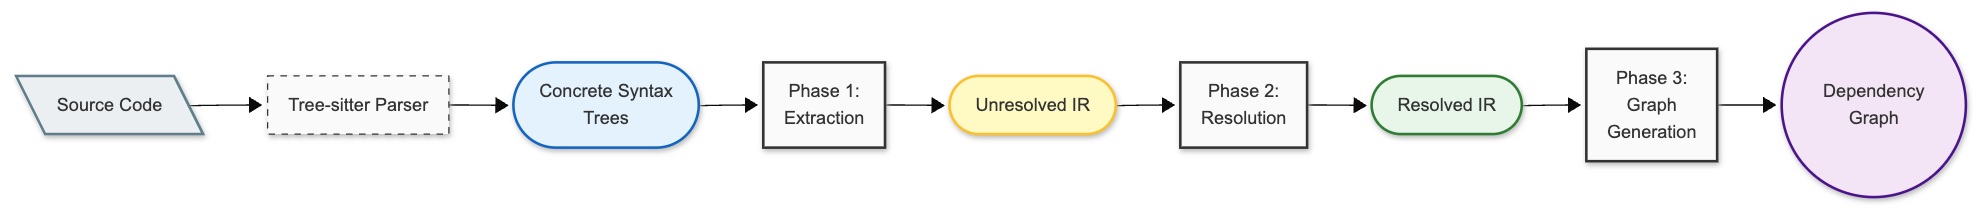
\includegraphics[width=\textwidth]{images/analysis_pipeline.png}
  \caption{The functional pipeline of the analyzer. Source code is
    parsed into a CST, mapped to an unresolved IR (Phase 1),
    semantically resolved (Phase 2), and finally flattened into a
  Dependency Graph (Phase 3).}
  \label{fig:analysis_pipeline}
\end{figure}

Modeling the system as a functional pipeline allows us to reason
about its structural correctness: each phase receives a well-formed
input and guarantees the production of an equally valid output
(\textit{Type Safety}). This separation of concerns ensures the
overall semantic consistency of the architecture, making it trivial
to add support for new languages by simply plugging in new extraction
heuristics for Phase 1, without touching the core resolution engine.

\subsection{Scope and Limitations}
It is important to emphasize that this tool is designed exclusively
for \textbf{static} architectural analysis. The extraction and
resolution of dependencies are based solely on the source code as it
is written. Consequently, the analyzer does not track or resolve
dynamic behaviors that occur at runtime, such as reflection, advanced
duck-typing, or dynamic dispatch mechanisms. The graph represents the
architecture explicitly declared by the developer, offering a
deterministic view of the codebase's structural dependencies.

\section{Organization of the Thesis}
\todo{Complete and refine the outline of the thesis
chapters once the structure is finalized}

\todo[inline]{The remainder of this thesis is organized as follows:
  Chapter 2 reviews the state of the art and the existing tools in
  the context of static analysis and parsing.
  Chapter 3 introduces the theoretical foundation of our
  language-agnostic Intermediate Representation (IR).
  Chapter 4 details the design and implementation of the extraction
  and resolution pipelines.
  Chapter 5 presents the evaluation of our tool across different
  benchmark projects and programming languages.
  Finally, Chapter 6 draws the conclusions and outlines potential
directions for future work.}
